\section{Contrôle de jobs dans le shell}
La section suivante explore les commandes et l'utilisation du contrôle de jobs dans le shell. 
\newline
\newline
Lorsqu'une commande est suivie d'une esperluette (\&), elle s'exécute en background (arrière-plan). 
Chaque travail en arrière-plan est identifié par un numéro unique attribué par le shell. Par exemple :

\begin{lstlisting}[style=blackstyle]
$ sleep 50 & 
[1] 112	# Job 1 : process cat avec PID 112
$ sleep 55 &
[2] 114	# Job 2 : process ls avec PID 114
\end{lstlisting}
Le numéro qui suit le numéro de travail est le PID processus créé pour exécuter la commande, ou, dans le cas d'un pipeline, le PID du dernier processus du pipeline. Afin de faire référence à un job particulier, la notation \verb|%num| est nécessaire, où "num" est le numéro de job assigné par le shell.
\newline
\newline
La commande intégrée du shell \texttt{jobs} liste tous les jobs en arrière-plan :
\begin{lstlisting}[style=blackstyle]
$ jobs
[1]- Running sleep 50 & 
[2]+ Running sleep 55 &
\end{lstlisting}

À ce stade, le shell est le processus en avant-plan pour le terminal. Comme seul un processus en avant-plan peut lire l'entrée du terminal et recevoir 
des signaux générés par le terminal, il est parfois nécessaire de déplacer un travail en arrière-plan vers l'avant-plan. 
Cela se fait en utilisant la commande intégrée du shell \texttt{fg} :
\begin{lstlisting}[style=blackstyle]
$ jobs
$ fg %1
sleep 50 & 
\end{lstlisting}

Comme le montre cet exemple, le shell réaffiche la ligne de commande d'un travail chaque fois que le travail est déplacé entre l'avant-plan 
et l'arrière-plan. Ci-dessous, nous verrons que le shell le fait également chaque fois que l'état du travail change en arrière-plan.
\newline
Lorsqu'un travail s'exécute en avant-plan, nous pouvons le suspendre en utilisant le caractère de suspension du terminal 
(généralement Control-Z), qui envoie le signal SIGTSTP au groupe de processus en avant-plan du terminal :
\begin{lstlisting}[style=blackstyle]
Tapez Control-Z
[1]+ Stopped sleep 50 & 
\end{lstlisting}

Après avoir tapé Control-Z, le shell affiche la commande qui a été arrêtée en arrière-plan. Si nécessaire, nous pouvons utiliser la commande \texttt{fg} pour reprendre le travail en avant-plan, ou utiliser la commande \texttt{bg} pour le reprendre en arrière-plan. Dans les deux cas, le shell reprend le travail arrêté en lui envoyant un signal SIGCONT :
\begin{lstlisting}[style=blackstyle]
$ bg %1
[1]+ sleep 50 &  
\end{lstlisting}

Nous pouvons arrêter un travail en arrière-plan en lui envoyant un signal SIGSTOP :

\begin{lstlisting}[style=blackstyle]
$ kill -STOP %1
[1]+ Stopped sleep 50 & 
$ jobs
[1]+ Stopped sleep 50 & 
[2]- Running sleep 55 &
$ bg %1    #  Redemarrer le job  en arriere-plan
[1]+ sleep 50 & 
\end{lstlisting}


\subsection{Démonstration du contrôle de jobs}

Afin de mieux comprendre le comportement et l'organisation du shell en ce qui concerne les commandes de contrôle de jobs, le programme ci-dessous permettra de mieux saisir ces notions.

Ce programme de démonstration vise à reproduire le comportement des jobs gérés par un shell, mettant particulièrement en lumière la manière dont les processus dans un pipeline peuvent être organisés en un job.
Cette démonstration est conçue pour illustrer le comportement de plusieurs instances s'exécutant dans un pipeline, comme illustré ci-dessous :


\begin{lstlisting}[style=blackstyle]
$ ./job | ./job 
\end{lstlisting}

\begin{lstlisting}[caption={jobControl.c}, label={jobControl.c}]
#include <stdio.h>
#include <stdlib.h>
#include <unistd.h>
#include <signal.h>
#include <sys/types.h>

void sigint_handler(int signo) {
	fprintf(stderr,"PID: %d: J'ai recu SIGINT\n", getpid());
}

void sigtstp_handler(int signo) {
	fprintf(stderr,"PID: %d: J'ai recu SIGTSTP\n",
    getpid(), getppid(), getpgrp(), getsid(0));
	raise(SIGSTOP);  // Suspendre le process
}

void sigcont_handler(int signo) {
	fprintf(stderr,"PID: %d: J'ai recu SIGCONT\n",
    getpid(), getppid(), getpgrp(), getsid(0));
	if (isatty(STDIN_FILENO) && (getpid() == getpgrp())) {
    // Print groupe foreground ssi stdin est un terminal et que
    // le process est un leader de groupe
    	fprintf(stderr,"Groupe en foreground: %d\n", tcgetpgrp(STDIN_FILENO));
	}
}

int main() {
	// Handlers pour SIGINT, SIGTSTP et SIGCONT
	signal(SIGINT, sigint_handler);
	signal(SIGTSTP, sigtstp_handler);
	signal(SIGCONT, sigcont_handler);

    if (isatty(STDIN_FILENO) && (getpid() == getpgrp())) {
    // Print groupe foreground ssi stdin est un terminal et que
    // le process est un leader de groupe
    	fprintf(stderr,"Groupe en foreground: %d\n", tcgetpgrp(STDIN_FILENO));
	}

	fprintf(stderr,"Je suis le process: PID: %d, PPID: %d, PGID: %d, SID: %d\n",
    getpid(), getppid(), getpgrp(), getsid(0));

	while (1) {
    	pause();
	}

	return 0;
}
\end{lstlisting}

La session de shell suivante démontre l'utilisation du programme.
\newline

\begin{lstlisting}[style=blackstyle]
$ echo $$  # PID du shell
2062
$ ./job | ./job & 
[1] 4511
Je suis le process: PID: 4511, PPID: 2062, PGID: 4510, SID: 2062
Groupe en foreground: 2062
Je suis le process: PID: 4510, PPID: 2062, PGID: 4510, SID: 2062
\end{lstlisting}

À partir du résultat ci-dessus, nous pouvons voir que le shell est le processus en foreground (\texttt{tcgetpgrp()})
pour le terminal. On remarque aussi que tous les processus sont dans la même session que le shell et dans un groupe différent du shell.
\newline
Ramenons maintenant ce job en foreground à l'aide de \texttt{fg}. Et tapons CTRL-C pour envoyer un signal SIGINT

\begin{lstlisting}[style=blackstyle]
$ fg
./job | ./job
# Tapez Control-C pour generer SIGINT
PID: 4511: J'ai recu SIGINT
PID: 4510: J'ai recu SIGINT
\end{lstlisting}

À partir de la sortie ci-dessus, nous voyons que le signal SIGINT a été délivré à tous les
processus dans le groupe en foreground du terminal (à savoir le job avec les programmes).
Le programme ne s'arrête pas puisqu'il gère ce signal.
\newline
Utilisons maintenant SIGTSTP à l'aide de Control-Z

\begin{lstlisting}[style=blackstyle]
# Tapez Control-Z pour generer SIGTSTP
PID: 4511: J'ai recu SIGTSTP
PID: 4510: J'ai recu SIGTSTP
[1]+  Stopped             	./job | ./job
\end{lstlisting}

Tous les processus du job sont maintenant à l'arrêt. Le shell devient donc le groupe en foreground et a la main
sur le terminal.
\newline
Relançons maintenant le job en background à l'aide de \texttt{bg}.

\begin{lstlisting}[style=blackstyle]
$ bg
[1]+ ./job | ./job &
PID: 4511: J'ai recu SIGCONT
PID: 4510: J'ai recu SIGCONT
Groupe en foreground: 2062
\end{lstlisting}

On remarque donc que tous les processus du job ont été délivrés SIGCONT, et reprennent leurs exécutions.
\newline
Pour nettoyer la démonstration, la commande "kill" peut être utilisée.
\begin{lstlisting}[style=blackstyle]
$ kill %1
[1]- Terminated ./job | ./job
\end{lstlisting}

\subsubsection{Schéma récapitulatif}

Le schéma ci-dessous illustre les differents états d'un processus sous le fonctionnement de contrôle de jobs.

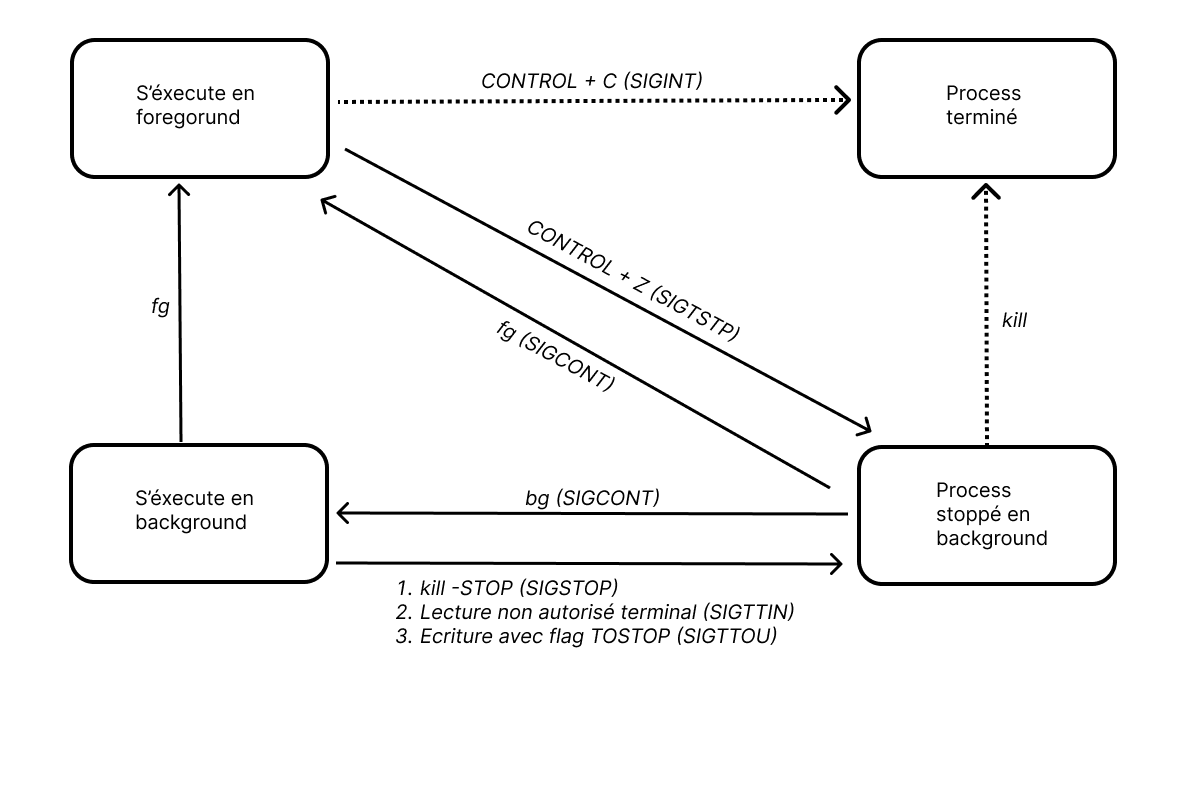
\includegraphics[width=1\textwidth]{img/jobControl.png}





